\documentclass[11pt]{article}

\newcommand{\numpy}{{\tt numpy}}    % tt font for numpy

\topmargin -.5in
\textheight 9in
\oddsidemargin -.25in
\evensidemargin -.25in
\textwidth 7in
\usepackage{tikz}
\usetikzlibrary{automata,positioning}


\begin{document}

% ========== Edit your name here
\author{ Asst. Prof. Dr. Çiğdem Turhan\\Res. Asst. Burcu Alakuş}
\title{HOMEWORK I\\CMPE 326 - Formal Languages \& Automata\\  Due Date: April 12, 2020}
\date{\vspace{-5ex}}
\maketitle

\medskip

% ========== Begin answering questions here
\begin{enumerate}

\item
DFA (30p)

a) Convert the language L into the corresponding DFA, where L is the set of the strings with at least two a's and at most one b. (20p)\\\\
b) Describe the language recognized by the following DFA. (10p)\\\\
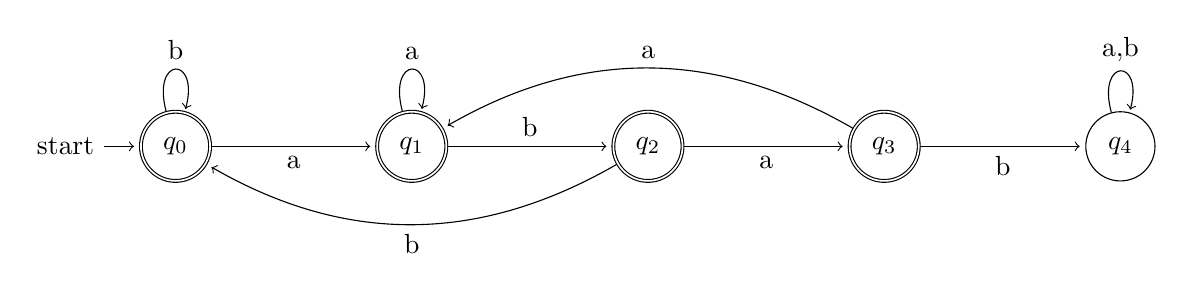
\begin{tikzpicture}[shorten >=2pt,node distance=3cm,on grid,auto] 
   \node[state,initial,accepting] (q_0)   {$q_0$}; 
   \node[state,accepting] (q_1) [right=of q_0] {$q_1$};
   \node[state,accepting] (q_2) [right=of q_1] {$q_2$};
   \node[state,accepting](q_3) [right=of q_2] {$q_3$};
   \node[state](q_4) [right=of q_3] {$q_4$};
    \path[->] 
    (q_0) edge  [loop above] node {b} (q_0)
          edge  node [swap] {a} (q_1)
    (q_1) edge  node  {b} (q_2)
          edge [loop above] node {a} ()
    (q_2) edge  node [swap] {a} (q_3) 
          edge [bend left, below] node {b} (q_0)
    (q_3) edge  node [swap] {b} (q_4) 
          edge [bend right, above] node {a} (q_1)
    (q_4) edge [loop above] node {a,b} (q_4);
\end{tikzpicture}


\item
NFA (35p)

a) Construct an NFA of the language L, where L is the set of strings over the alphabet $\Sigma$=$\{$0,1,2$\}$ such that every 0 is followed by exactly two 1's and every 2 is followed either by 01 or 10. (10p)\\\\
b) Convert the following NFA into the corresponding DFA. (25p)\\
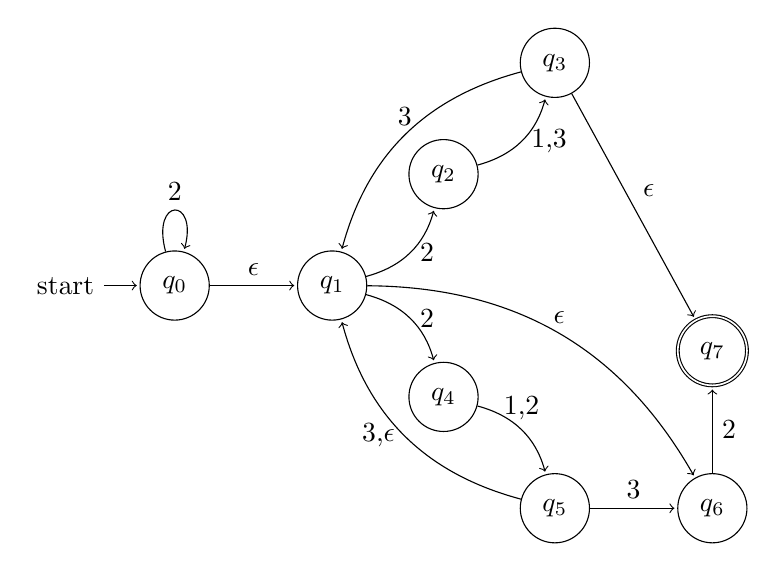
\begin{tikzpicture}[shorten >=1pt,node distance=2cm,on grid,auto] 
   \node[state,initial] (q_0)  {$q_0$}; 
   \node[state](q_1) [right=of q_0] {$q_1$};
   \node[state](q_2) [above right=of q_1] {$q_2$};
   \node[state](q_3) [above right=of q_2] {$q_3$};
   \node[state](q_4) [below right=of q_1] {$q_4$};
   \node[state](q_5) [below  right =of q_4] {$q_5$};
   \node[state](q_6) [right=of q_5] {$q_6$};
   \node[state,accepting](q_7) [above=of q_6] {$q_7$};
    \path[->] 
    (q_0) edge [loop above] node {2} (q_0)
          edge node {$\epsilon$} (q_1)
    (q_1) edge  [bend left, above] node {$\epsilon$} (q_6)
          edge [bend right, right] node  {2} (q_2)
          edge [bend left, right]node {2} (q_4)
    (q_2) edge  [bend right, right] node {1,3} (q_3) 
    (q_3) edge [bend right, above] node {3} (q_1)
          edge node {$\epsilon$} (q_7)
    (q_4) edge [bend left, above] node {1,2} (q_5)
    (q_5) edge [bend left,left] node {3,$\epsilon$} (q_1) edge node {3} (q_6)
    (q_6) edge node [right] {2} (q_7);

\end{tikzpicture}
\\
\item
DFA Minimization (25p)

Minimize the following DFA: \\
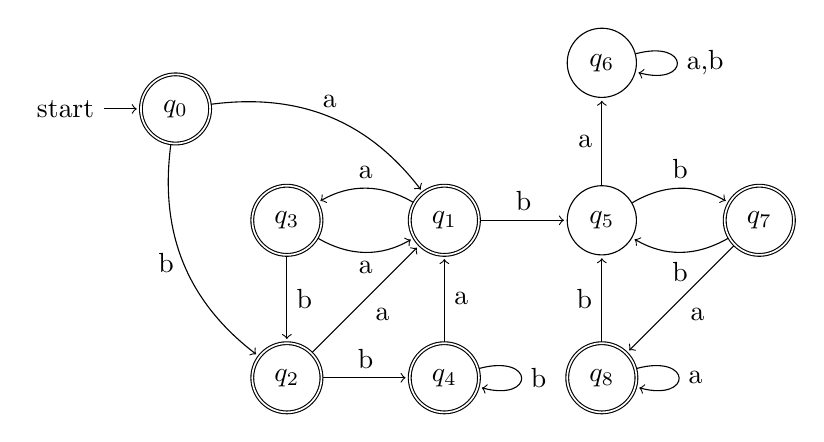
\begin{tikzpicture}[shorten >=1pt,node distance=2cm,on grid,auto] 
   \node[state,initial,accepting] (q_0)  {$q_0$}; 
   \node[state,accepting](q_3) [below right=of q_0] {$q_3$};
   \node[state,accepting](q_1) [right=of q_3] {$q_1$};
   \node[state,accepting](q_2) [below=of q_3] {$q_2$};
   \node[state,accepting](q_4) [right=of q_2] {$q_4$};
   \node[state](q_5) [right=of q_1] {$q_5$};
   \node[state](q_6) [above=of q_5] {$q_6$};
   \node[state,accepting](q_7) [right=of q_5] {$q_7$};
   \node[state,accepting](q_8) [below=of q_5] {$q_8$};
    \path[->] 
    (q_0) edge [bend right,left] node {b} (q_2)
          edge [bend left,above] node  {a} (q_1)
    (q_1) edge  [bend right, above] node {a} (q_3)
          edge node  {b} (q_5)
    (q_2) edge  node [swap] {a} (q_1) 
          edge node {b} (q_4)
    (q_3) edge  [bend right, below] node {a} (q_1)
          edge node {b} (q_2)
    (q_4) edge [loop right] node {b} (q_4)
          edge node [swap] {a} (q_1)
    (q_5) edge [bend left,above] node {b} (q_7)
          edge node {a} (q_6)
    (q_6) edge [loop right] node {a,b} (q_6)
    (q_7) edge [bend left,below] node {b} (q_5)
          edge node {a} (q_8)
    (q_8) edge [loop right] node {a} (q_8)
          edge node {b} (q_5);
\end{tikzpicture}


\item
Regular Expression (10p)

Write a regular expression for the set of strings consist of alternating 0's and 1's (=strings with no consecutive 0's or 1's)
\end{enumerate}

\end{document}
\grid
\grid